%?????????????????
\documentclass[11pt, letterpaper, onecolumn, oneside, final]{article}

\usepackage{lab}
\usepackage{soul}

\newfontfamily{\consolas}{Consolas}
[Extension = .ttf]
%\usepackage{fontspec}

\DocumentTitle {Lab 5A}
\DocumentSubtitle {Web-Scraping!}
% End of preamble

%%%%%%%%%%%%%%%%%%%%%%%%%%%%%%%%%%%%%%%%%%%%%%%%%%%%%%%%%%%%%%%%%%%%%%%

\begin{document}
\maketitle

% MAKE SURE TO SAVE THIS LAB IN A LABS FOLDER
% LISTS/FOR LOOP QUESTIONS -------------------------------------------
\section{Introduction.} In this lab you will be using what you have learned in class about web scraping as well as a few new things presented in this lab to complete exercises that involve pulling and analyzing data from the web in order to sharpen you skills with {\consolas beautifulSoup}.

\section{Installation:}
    First install {\consolas BeautifulSoup} from Thonny's package manager, following these steps:
\begin{enumerate}
    \item Open Thonny. Click {\consolas Tools > Manage Packages...}
    \item In the search bar, type {\consolas bs4}. Click {\consolas Install} and wait for it to be installed. You will be able to tell when it is done.
\end{enumerate}
This is the general process to install most packages in Thonny. At the top of your {\consolas lab5A.py} file, make sure you have the lines:
\begin{center}
\colorbox{lightgray}{\parbox{.4\textwidth}{\consolas from bs4 import BeautifulSoup\\
import requests}}
\end{center}
Any time you want to web-scrape using {\consolas BeautifulSoup} you need these lines at the top of your file. \\
Start by  downloading {\consolas lab5A.py} file from the Piazza page and open it in Thonny.

    \item In this lab, we will be scraping data off of the Hamilton College site. We will start by explaining a little bit about HTML, the coding language used to create webpages.
    \\
    
    
    
    %\colorbox{lightgray}{\parbox{.8\textwidth}{\consolas <div class="intro"> \\ \hspace*{8mm}Hamilton offers 43 majors (we call them concentrations) and 
    %\hspace*{8mm}57 total areas of study. \\ </div>}}
\section{Understanding HTML.} To begin, we will be introducing the important pieces of HTML code, using the graphic below.\\\\
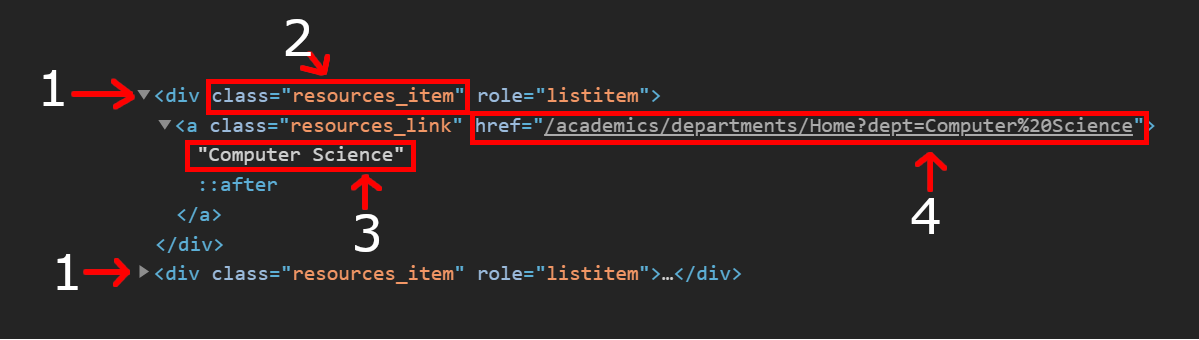
\includegraphics[scale = .5]{tags_final}
\\\\
    Most lines contain structures called \textbf{tags}, which start with {\consolas <tagname>} and ends with {\consolas </tagname>}. In the above example the {\consolas div} tag (labeled with a 1) which is used to organize sections of code, starts with {\consolas <div>} and ends with {\consolas </div>}. In between the opening tag and the closing tag is the \textbf{text} of the tag. This can contain text, or other tags. In this example, there is another tag: {\consolas <a>}. The text within this {\consolas <a>} tag is {\consolas "Computer Science"} (labeled with a 3). Another important element of tags is \textbf{class}, which are used to organize various tags, and will be useful while scraping for searching for specific lines of code. (You may also see tags with \textbf{id} in addition to (or instead of) class. For our purposes, we can treat them the same). The tag's \textbf{class} and \textbf{id} are found \textbf{inside} the opening tag. In this case, this tag's \textbf{class} is {\consolas resources\_item} (labeled with a 2), and it's \textbf{text} is the {\consolas <a>} tag. Meanwhile the {\consolas <a>} tag's \textbf{class} is {\consolas resources\_link}. Another important thing to note is {\consolas href}, which you can see inside the {\consolas <a>} tag. The {\consolas href} piece (labeled with a 4) is used to provide links to other pages, as well as images, video, and other media. 
\section{What to do.}
\begin{enumerate}    
    \item Now that you have somewhat of an idea of the structure of HTML, open up the following webpage: 
    \textcolor{blue}{\underline{https://www.hamilton.edu/academics/areas-of-study}}. By right clicking on the page and selecting `inspect', you can see the HTML code for whatever you clicked on (as well as the rest of the page). If you are using a Mac, you have to right click with \textbf{two} fingers. If this still does not work, ask your TA and they will help you. 
    
    \item Now go to the {\consolas lab5A.py} file. Notice that the {\consolas url} string is empty. This is where you put the link to the webpage you want to begin scraping. For now, put the link for Hamilton's Areas of Study page into the url string. The following line then gets the source code:
    \begin{center}
        \colorbox{lightgray}{\parbox{.48\textwidth}{\consolas source\_code =  requests.get(url).text}}
    \end{center}
    This line then parses the code and gives it back in a format we can use BeautifulSoup to further parse:
    \begin{center}
        \colorbox{lightgray}{\parbox{.7\textwidth}{\consolas parsed\_code = BeautifulSoup(source\_code, "html.parser")}}
    \end{center}
    You should use these two lines whenever you want to scrape a new webpage. 
    
    \item The {\consolas find()} function can be used to find a tag within some code. Similarly, the {\consolas find\_all()} function can be used to find all occurences of a tag. For the following lines of code, predict the value of the output using the inspect element tool in your browser. Then use the program skeleton to check your answers. (Often the output will be very long, it is sufficient to write down only the first line or two OR a description of what the output is.)
    \begin{enumerate}
        \item \colorbox{lightgray}{\parbox{.43\textwidth}{\consolas header = parsed\_code.find("head")}}\\\\
        % <head> 
        % <meta name="keywords" content="Areas of Study, Majors, Minors, Hamilton College, Academics, Hamilton major"> i.e all the header code
        
        \item \colorbox{lightgray}{\parbox{.36\textwidth}{\consolas title = header.find("title")}}\\\\
        % <title>Academics - Areas of Study - Hamilton College</title>
        
        \item \colorbox{lightgray}{\parbox{.23\textwidth}{\consolas title = title.text}} \\\\ % Academics - Areas of Study - Hamilton College
        
        \item \colorbox{lightgray}{\parbox{.34\textwidth}{\consolas link1 =  header.find("link")}} \\\\
        % <link rel="mask-icon"  href="/assets/images/favicons/safari-pinned-tab.svg?v=0.0.1" color="#002f86">
        
        \item \colorbox{lightgray}{\parbox{.33\textwidth}{\consolas link2 =  link1.find("link")}} \\\\ % NONE
        
        
        \item \colorbox{lightgray}{\parbox{.28\textwidth}{\consolas answer = answerList[1]}}\\\\ % Second link in the header
        
        \item \colorbox{lightgray}{\parbox{.3\textwidth}{\consolas answer = answer['color']}}\\\\
        
        \item \colorbox{lightgray}{\parbox{.39\textwidth}{\consolas body = parsed\_code.find("body")}}\\\\ % Code body
        
        \item \colorbox{lightgray}{\parbox{.34\textwidth}{\consolas body2 = header.find("body")}}\\\\ % None
        
        \item \colorbox{lightgray}{\parbox{.41\textwidth}{\consolas link3 = parsed\_code.find("link")}}\\\\ % <link rel="mask-icon"  href="/assets/images/favicons/safari-pinned-tab.svg?v=0.0.1" color="#002f86"> (first link tag in entire code)
        
        \item \colorbox{lightgray}{\parbox{.83\textwidth}{\consolas div1 = body.find("div", class\_="page\_wrapper js-navigation\_push")}} \\\\ 
        % gets main body of code
        
        \item \colorbox{lightgray}{\parbox{.51\textwidth}{\consolas div2 = body.find("div", class\_="footer")}}
        % gets the footer
        
    \end{enumerate}
    
    \item Now, given the strings below, write code that will scrape the website in order to produce these strings. This will require some understanding of the HTML on the page. This can get a little tricky, so feel free to ask a professor or TA for help.
    \begin{enumerate}
        \item {\consolas 198 College Hill Road, \\Clinton, \\NY, \\13323}\\\\ % Can be grabbed in the footer        
        \item {\consolas <img src="/assets/images/BH-logo.png" alt="Campaign Header graphic" height="25" border="0">}\\\\
        \item {\consolas Archaeology}\\\\
        \item {\consolas "/academics/departments/Home?/dept=Computer\%20Science"}\\\\
        \item {\consolas "**"}\\\\
    \end{enumerate}
    
    \item Now use the {\consolas find\_all()} to get a list of all the department names and the links ({\consolas hrefs}) to the corresponding department page. (Hint: The value in {\consolas href} is not the whole link. What would you combine it with to get the actual link?)
    
    \item The departments on this site are labeled with asterisks to denote that they are offered as only a minor (1 asterisk) or if they are not available for a major or a minor (2 asterisks). Using your list from the previous exercise, create three new lists, based on the number of asterisks that follow the department name. 
    
    \item Pick a department. Navigate to their page by using the {\consolas requests} and {\consolas BeautifulSoup} lines we used earlier, but now with the new link that you found in exercise 5. Once you are on that page, there should be a section titled ``Sampling of Courses". Try scraping all of those courses, their numbers, and descriptions, printing them all out. This will be difficult and will require you to look deeply at the HTML code. Ask a professor or TA if you get stuck or need help.
    
    \item As a greater challenge than above try scraping the number, description, and name of all the courses in a given department. This can be done by expanding on the exercises above but using the link from the ``View All Courses" button on the page for that area of study to get to the webpage that lists off all courses in that department. This will require more steps than the previous exercises, and will be rather difficult. Try your best and ask questions when you have them!
    
\end{enumerate}
% scrape the academics page with areas of study
% get each major and its corresponding link
% write a function that allows the user to search for a department & bring you to the URL if it is there, or report that we don't have it
% maybe sort by what we have as majors, minors, or neither?
\end{document}